\documentclass{mta}

\begin{document}

\title{修論抄録集フォーマット(\LaTeX{}版)}
\subtitle{副題があればここに書く} % 副題が無ければコメントに

\etitle{A \LaTeX{} format for Master Thesis Abstract}
\esubtitle{Write english subtitle if available} % 副題が無ければコメントに

\author{拓殖 太郎}
\major{情報・デザイン工学}
\supervisor{教授 館町 一郎}
\coexaminer{准教授 小日向 二郎}



\maketitle

\chapter{はじめに}

修士論文の抄録を\LaTeX{}\cite{latex}で作成するためのスタイルファイルを作成した.
問題点があれば修正するので蓑原
\footnote{\url{mailto:minohara@cs.takushoku-u.ac.jp}}
に連絡して欲しい.

基本的に標準の\LaTeX{}コマンドをそのまま使うことができる.
本稿は,スタイルファイルを実際に使って記述しているので参考にして欲しい.

なお,スタイル自体は異なるが,本稿の説明の一部は
「情報処理学会研究報告の準備方法(2018年10月29日版)」\cite{ipsjreport}をもとにしている.

\chapter{修論抄録集フォーマットの使い方}

\section{準備}

スタイルファイル一式は次のGitHub リポジトリから入手できる
\url{https://github.com/minohara/MTA}

このリポジトリには次のファイルが含まれている.

\begin{itemize}
    \item \verb|mta.cls| : スタイルファイル
    \item \verb|mta.tex| : 本稿のソースファイル%
    \footnote{このファイルを直接書き換えるのではなく,提出するファイル名でコピーしてから,参照しながら記述していくことを勧める}
    \item \verb|mta.pdf| : 本稿の出力ファイル
    \item \verb|mta.bib| : BiB\TeX{}のデータベースのサンプル
    \item \verb|ipsjunsrt.bst| : 情報処理学会のBiB\TeX{}スタイルファイル
\end{itemize}

\section{ソースファイルの構成}

抄録のソースファイルは次のような形式で記述する.

\noindent
\hrulefill\\
\verb|\documentclass{mta}|\\
\quad 必要ならばユーザのマクロをここに記述\\
\verb|\begin{document}|\\
\verb|\title{表題(和文)}|\\
\quad 必要ならば \verb|\subitile{副題(和文)}|で副題を入れる\\
\verb|\etitle{表題(英文)}|\\
\quad 必要ならば \verb|\esubitile{副題(英文)}|で副題を入れる\\
\verb|\author{論文著者氏名}|\\
\verb|\majour{専攻名}|\\
\verb|\supervisor{指導教員の役職と氏名}|\\
\verb|\coexaminer{副査の役職と氏名}|\\
\verb|\chapter{|第1章の表題\verb|}|\\
\dots\dots\dots\dots\dots\\
\quad \verb|<本文>|\\
\dots\dots\dots\dots\dots\\
\verb|\end{document}|\\
\hrulefill


\section{本文}

\subsection{見出し}

節や小節の見出しには \verb|\chapter|, \verb|\section|, \verb|\subsection|といったコマンドを使用する.

\<「定義」,「定理」などについては,\verb|\newtheorem|で適宜環境を宣言し,そ
の環境を用いて記述する.

%4.2.2
\subsection{行送り}

2段組の左右の段で行の基準線の位置が一致することを原則としている.
そのため,章見出しなど,
行の間隔を他よりたくさんとった方が読みやすい場所では,
スタイルファイルが自動的にスペースを挿入する.
頁の境界に何がくるかによってスペースが変化するので,特に編集途中では 
\verb|\vspace| や \verb|\vskip| を用いたスペースの調整を行なわないようにすること.

\subsection{フォントサイズ}
フォントサイズは,スタイルファイルによって自動的に設定されるため,
基本的には著者が自分でフォントサイズを変更する必要はない.


\subsection{句読点}
句点には全角の「.」,
読点には全角の「,」を用いる.
ただし英文中や数式中で「.」や「,」を使う場合には,
半角文字を使う.「。」や「、」は使わない.

\subsection{全角文字と半角文字}
全角文字と半角文字の両方にある文字は次のように使い分ける.

\begin{enumerate}
\item 括弧は水平方向の基準線が異なるので,和文中では原則として全角の「(」と「)」を用いる.
ただし,括弧の内または外が英文の場合,図表見出し,書誌データなどでは,半角の「(」と「)」を用いる.

\item 英数字,空白,記号類は半角文字を用いる.ただし,句読点に関しては,
前項で述べたような例外がある.

\item カタカナは全角文字を用いる.

\item 引用符では開きと閉じを区別する.
開きには \verb|``| を用い,閉じには\verb|''| を用いる.
\end{enumerate}

\subsection{箇条書}
標準的な \verb|enumerate|,
\verb|itemize|, \verb|description| の環境を用いる.

\subsubsection{enumerateの例}

\begin{enumerate}
    \item enumerate
    \item itemize
    \item description
\end{enumerate}

\subsubsection{itemizeの例}

\begin{itemize}
    \item enumerate
    \item itemize
    \item description
\end{itemize}

\subsubsection{descriptionの例}

\begin{description}
    \item[enumerate] 番号付きリスト
    \item[itemize] 番号なしリスト 
    \item[description] 見出し付きリスト
\end{description}
\subsection{脚注}

脚注は \verb|\footnote| コマンドを使って書くと,
\footnote{脚注の例.}のような参照記号を付けてページごとに
脚注が生成される.

脚注をつけた位置と脚注本体とを別の段に置く場合には,\verb|\footnotemark| コマンドや \verb|\footnotetext| コマンドを使う.

\section{数式}

\subsection{本文中の数式}

本文中の数式は \verb|$| と \verb|$|, \verb|\(| と \verb|\)|, あるいは \verb|math| 環境のいず
れかで囲む.

\subsection{別組の数式}

別組数式(displayed math)については \verb|$$| と \verb|$$| は使用せずに,
\verb|\[| と \verb|\]| で囲むか,
\verb|displaymath|, \verb|equation|, \verb|eqnarray| のいずれかの環境を用いる.

\subsection{eqnarray環境}

互いに関連する別組の数式が2行以上連続して現れる場合には,
単に\verb|\[| と \verb|\]|,
あるいは \verb|\begin{equation}| と\verb|\end{equation}| で囲った数式を書き並べるのではなく,
\verb|\begin|\allowbreak\verb|{eqnarray}| と \verb|\end{eqnarray}| を使って,
等号(あるいは不等号)の位置で縦揃えを行なった方が読みやすい.

\section{図}

\begin{figure}[tb]
    \setbox0\vbox{
    \hbox{\verb|\begin{figure}[tb]|}
    \hbox{\quad \verb|<|図本体の指定\verb|>|}
    \hbox{\verb|\caption{<|図のタイトル\verb|>}|}
    \hbox{\verb|\label{| $\ldots$ \verb|}|}
    \hbox{\verb|\end{figure}|}
    }
    \fbox{\box0}
    \caption{図の形式}
    \label{fig:single}
\end{figure}
\begin{figure}[tb]
    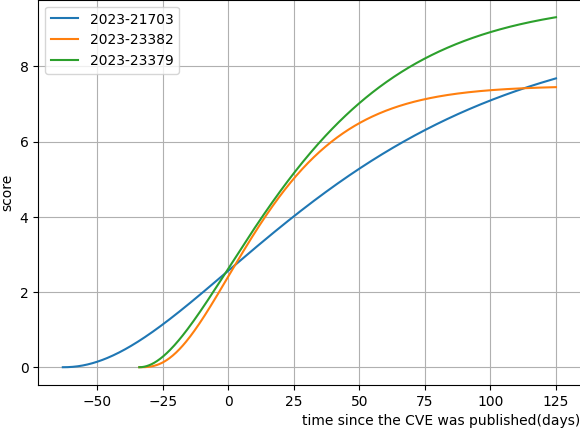
\includegraphics[width=0.9\linewidth]{image.png}
    \caption{画像の読み込みの例}
    \label{fig:include}
\end{figure}


\begin{table}[tb] 
    \caption{表の例} 
    \label{tab:example}
    \begin{tabular}{l|lll}\hline\hline
    & column1 & column2 & column3 \\\hline
    row1 &	item 1,1 & item 2,1 & ---\\
    row2 &	---      & item 2,2 & item 3,2 \\
    row3 &	item 1,3 & item 2,3 & item 3,3 \\
    row4 &	item 1,4 & item 2,4 & item 3,4 \\\hline
    \end{tabular}
    \end{table}
    

図は,\figref{fig:single} の形式で指定する.
位置の指定に \verb|h| は使わないほうがよい.
図のタイトルは,\verb|\caption| で入れる.
図の参照は \verb|\figref{<|ラベル\verb|>}| を用いて行なう.

画像ファイルを読み込む場合は \verb|\includegraphics|を使う.
図を拡大または縮小するときは縦横比を変えないように\verb|width|か\verb|height|のいずれか一方だけを指定する.

\section{表}

表の罫線を少なくすると仕上がりがすっきりする.お勧めは,
\tabref{tab:example}のように,
一番上の罫線には二重線を使い,左右の端には縦の罫線をつけない.

表のタイトルは表の上に\verb|\caption|で入れる.
表の参照は \verb|\tabref{<|ラベル\verb|>}| のように記述する.


\chapter{参考文献}

\section{参考文献の参照}

本文中で参考文献を参照する場合には\verb|\cite|を使用する.
参照されたラベルは参照順に番号付けられて,上付きで表示される.
%
\begin{quote}
文献 \verb|\cite{okumura}| は\LaTeX の総合的な解説書である.
\end{quote}
%
と書くと;
%
\begin{quote}
文献\cite{okumura}は\LaTeX の総合的な解説書である.
\end{quote}
%
が得られる.

\section{参考文献リスト}

参考文献リストは,BiB\TeX と 情報処理学会のスタイル
\verb+ipsjunsrt.bst+(参照順)
を用いて作ることを想定している.

Bib\TeX{}形式のデータはCiNii(\url{https://cir.nii.ac.jp/})
やIEEE Xplore(\url{https://ieeexplore.ieee.org/Xplore/home.jsp})
などで文献を検索したときに入手できるが,
自分が読んだ論文を Mendeley(\url{https://www.mendeley.com/download-reference-manager/})のような
文献管理システムで管理しておくと便利である.

\bibliographystyle{ipsjunsrt}
\bibliography{mta}
\end{document}